%% Shared body of the manuscript, part 2.
\section{The average number of critical vertices}\label{sec:jump}

Throughout this section $G$ is a graph of order $n\ge1$ and
$\gamma=\gamma(G)$. For $\gamma\le j\le n$ the family $\Dom_j(G)$ is
nonempty, and we write $c_j$ and $v_j$ for the mean and the variance of
$a(S)$ when $S$ is chosen uniformly at random from $\Dom_j(G)$:
\[
  c_j=\frac1{d_j}\sum_{S\in\Dom_j(G)}a(S),\qquad
  v_j=\frac1{d_j}\sum_{S\in\Dom_j(G)}\bigl(a(S)-c_j\bigr)^2 .
\]
In this notation the identity~\eqref{eq:incidence} reads
\begin{equation}\label{eq:mean}
  j-c_j=(n-j+1)\,\frac{d_{j-1}}{d_j}\qquad(\gamma\le j\le n).
\end{equation}
In particular $j-c_j>0$ for $\gamma<j\le n$, and $d_{j-1}\le d_j$ if and only
if $c_j\ge 2j-n-1$.

\begin{lemma}\label{lem:valley}
Let $\gamma<i<n$. If $d_{i-1}\ge d_i<d_{i+1}$, then $c_{i+1}-c_i>2$.
\end{lemma}

\begin{proof}
By~\eqref{eq:mean}, $c_i=i-(n-i+1)d_{i-1}/d_i\le 2i-n-1$ and, as $n-i>0$,
$c_{i+1}=i+1-(n-i)d_i/d_{i+1}>2i+1-n$.
\end{proof}

\begin{lemma}\label{lem:cov}
For $\gamma<j\le n$,
\[
  (j-c_j)\,(c_j-c_{j-1})\le v_j .
\]
\end{lemma}

\begin{proof}
Consider again the pairs $(S',S)$ with $S'\in\Dom_{j-1}(G)$,
$S\in\Dom_j(G)$ and $S'\subset S$. By Lemma~\ref{lem:basic}(ii),
$a(S)\le a(S')$ for each such pair. Summing over all pairs, and using that
each $S$ occurs in $j-a(S)$ pairs and each $S'$ in $n-j+1$ pairs, we get
\[
  \sum_{S\in\Dom_j(G)}\bigl(j-a(S)\bigr)\,a(S)\;\le\;
  (n-j+1)\sum_{S'\in\Dom_{j-1}(G)}a(S') .
\]
The left-hand side equals $d_j\bigl((j-c_j)c_j-v_j\bigr)$, and the right-hand
side equals $(n-j+1)d_{j-1}c_{j-1}=d_j(j-c_j)c_{j-1}$ by~\eqref{eq:mean}.
Dividing by $d_j$ gives the claim.
\end{proof}

For an integer $h\ge0$ we say that $G$ satisfies condition $(\mathrm{H}_h)$ if
\begin{equation}\label{eq:H}
  2\gamma-|S|\;\le\;a(S)\;\le\;2\gamma+2h-|S|
  \qquad\text{for every dominating set $S$ of $G$.}
\end{equation}
By Corollary~\ref{cor:twosided}, every forest $F$ satisfies $(\mathrm{H}_h)$
with $h=\Gamma(F)-\gamma(F)$. We put
\[
  K_h=\left\lceil\frac{(h+1)^2}{4}\right\rceil .
\]

\begin{lemma}\label{lem:jump}
Let $G$ satisfy $(\mathrm{H}_h)$. Then $c_j-c_{j-1}\le 2$ for every $j$ with
$\gamma+K_h\le j\le n$.
\end{lemma}

\begin{proof}
Fix such a $j$; note that $j>\gamma$ because $K_h\ge1$. Put $L=2\gamma-j$ and
$x=c_j-L$. By~\eqref{eq:H}, $L\le a(S)\le L+2h$ for every $S\in\Dom_j(G)$, so
$0\le x\le 2h$. Averaging the pointwise inequality
$(a(S)-L)(L+2h-a(S))\ge0$ over $\Dom_j(G)$ gives
\begin{equation}\label{eq:variance}
  v_j\le x\,(2h-x) .
\end{equation}
Since $j-c_j=2(j-\gamma)-x$, we have the identity
\[
  2(j-c_j)-x(2h-x)=\bigl(x-(h+1)\bigr)^2+4(j-\gamma)-(h+1)^2 ,
\]
whose right-hand side is nonnegative because $j-\gamma\ge K_h\ge(h+1)^2/4$.
Together with Lemma~\ref{lem:cov} and~\eqref{eq:variance} this yields
$(j-c_j)(c_j-c_{j-1})\le v_j\le 2(j-c_j)$, and $j-c_j>0$.
\end{proof}

\section{Unimodality}\label{sec:unimodal}

\begin{theorem}\label{thm:main}
Let $G$ be a graph of order $n\ge1$ that satisfies $(\mathrm{H}_h)$ for some
integer $h\ge0$. If
\begin{equation}\label{eq:condition}
  n-\gamma(G)\ge 3K_h-7 ,
\end{equation}
then $D(G,x)$ is unimodal.
\end{theorem}

\begin{proof}
Let $\gamma=\gamma(G)$ and $A=\lfloor(n+2\gamma+1)/3\rfloor
=\gamma+\lfloor(n-\gamma+1)/3\rfloor$. As in the proof of
Corollary~\ref{cor:segments}(i), which uses only the lower bound
in~\eqref{eq:H}, we have $d_{j-1}\le d_j$ whenever $1\le j\le n$ and $j\le A$.
Condition~\eqref{eq:condition} is equivalent to
$\lfloor(n-\gamma+1)/3\rfloor\ge K_h-2$, that is, to
\begin{equation}\label{eq:A}
  A+2\ge\gamma+K_h .
\end{equation}

Suppose that $(d_0,\dots,d_n)$ is not unimodal. Then there are indices $k<i$
with $d_k>d_{k+1}$ and $d_i<d_{i+1}$; choose $k$ minimal and then $i$ minimal.
By the minimality of $i$ we have $d_{i-1}\ge d_i$, both when $i=k+1$ and when
$i>k+1$. The strict descent at $k$ shows that $k+1>A$, hence $i\ge k+1\ge
A+1\ge\gamma+1$, and $i<n$ because $d_{i+1}>0$. Lemma~\ref{lem:valley}
gives $c_{i+1}-c_i>2$. On the other hand $i+1\ge A+2\ge\gamma+K_h$
by~\eqref{eq:A}, so Lemma~\ref{lem:jump} gives $c_{i+1}-c_i\le2$, a
contradiction.
\end{proof}

\begin{proof}[Proof of Theorem~\ref{thm:criterion-intro}]
(i) This is Theorem~\ref{thm:main} together with
Corollary~\ref{cor:twosided}.

(ii) Let $F$ be a forest without isolated vertices such that $D(F,x)$ is not
unimodal, and write $\gamma=\gamma(F)$ and $K=K_h$. By~(i),
$n-\gamma\le 3K-8$. By Lemma~\ref{lem:ore}, $n\ge\gamma+\Gamma(F)=2\gamma+h$,
that is, $\gamma\le(n-\gamma)-h$. Therefore
\[
  n=(n-\gamma)+\gamma\le 2(n-\gamma)-h\le 6K-h-16 .
\]
Since $K_0=K_1=1$ and $K_2=3$, the right-hand side is at most $0$ when
$h\le2$, which is impossible. Hence $h\ge3$.

(iii) Since $K_h\le\bigl((h+1)^2+3\bigr)/4$, we have
$6K_h-h-16\le(3h^2+4h-20)/2$. If $2n\ge3h^2+4h-19$, then $n>6K_h-h-16$, and
$D(F,x)$ is unimodal by~(ii).
\end{proof}

\begin{corollary}\label{cor:gapthree}
Let $F$ be a forest with $\Gamma(F)-\gamma(F)\le3$. Then $D(F,x)$ is
unimodal.
\end{corollary}

\begin{proof}
By Lemma~\ref{lem:isolates} we may assume that $F$ has no isolated vertices.
Suppose that $D(F,x)$ is not unimodal. By
Theorem~\ref{thm:criterion-intro}(ii) the gap is $h=3$, so $K_h=4$,
$n\le5$, and $n\ge2\gamma(F)+3$ by Lemma~\ref{lem:ore}. Hence $\gamma(F)=1$
and $n=5$: some vertex is adjacent to the other four, and, $F$ being a
forest, $F$ is the star $K_{1,4}$. A dominating set of $K_{1,4}$ either
contains the centre or consists of the four leaves, so
\[
  D(K_{1,4},x)=x(1+x)^4+x^4=x+4x^2+6x^3+5x^4+x^5 ,
\]
which is unimodal. This contradiction proves the corollary.
\end{proof}

For gap at most two, Corollary~\ref{cor:gapthree} extends the theorem of
Beaton and Schoonhoven~\cite[Corollary~17]{BS} from trees to forests; the case
of gap three is new already for trees.

\section{Small trees and the case of gap four}\label{sec:small}

\subsection{Log-concavity for trees with at most \texorpdfstring{$\MaxLC$}{26} vertices}

\begin{theorem}\label{thm:small}
The domination polynomial of every tree with at most $\MaxLC$ vertices is
log-concave.
\end{theorem}

\begin{proof}
This is the result of an exhaustive computation over the $\TotalTreesLC$
isomorphism classes of trees with at most $\MaxLC$ vertices. The algorithms,
the completeness checks and the two independent implementations are described
in Appendix~\ref{app:computation}.
\end{proof}

To pass from trees to forests we use the classical fact that log-concavity is
preserved by products; see, for example, Stanley's survey~\cite{Stanley}. A
sequence $(a_k)_{k\in\mathbb Z}$ of nonnegative numbers with finitely many
nonzero terms has \emph{no internal zeros} if its support is an interval.

\begin{lemma}\label{lem:product}
Let $P$ and $Q$ be polynomials whose coefficient sequences are nonnegative,
log-concave and without internal zeros. Then the coefficient sequence of
$PQ$ has the same three properties.
\end{lemma}

\begin{proof}
Let $(a_k)$, $(b_k)$ and $(c_k)$ be the coefficient sequences of $P$, $Q$ and
$PQ$, extended by zero to all integer indices. A nonnegative log-concave
sequence $(a_k)$ without internal zeros satisfies
\begin{equation}\label{eq:tp2}
  a_i\,a_j\ge a_{i-1}\,a_{j+1}\qquad\text{for all } i\le j ,
\end{equation}
because, when the right-hand side is positive, the ratios $a_k/a_{k-1}$ are
positive and nonincreasing for $i\le k\le j+1$. Expanding the products shows
that
\[
  c_k^2-c_{k-1}c_{k+1}=\sum_{i<j}
  \bigl(a_i a_{j-1}-a_{i-1}a_j\bigr)\bigl(b_{k-j+1}b_{k-i}-b_{k-j}b_{k-i+1}\bigr),
\]
which is the Cauchy--Binet formula for a $2\times2$ minor of a product of two
matrices. Both factors of each summand are nonnegative by~\eqref{eq:tp2}.
Finally, the support of $(c_k)$ is the sumset of two intervals, hence an
interval.
\end{proof}

\begin{corollary}\label{cor:smallforest}
Let $F$ be a forest all of whose components have at most $\MaxLC$ vertices.
Then $D(F,x)$ is log-concave, and in particular unimodal.
\end{corollary}

\begin{proof}
The domination polynomial of a disjoint union is the product of the
domination polynomials of the components, and $D(K_1,x)=x$. By
Lemma~\ref{lem:basic}(i) the coefficient sequence of every domination
polynomial is nonnegative without internal zeros. The claim follows from
Theorem~\ref{thm:small} and Lemma~\ref{lem:product}, since a nonnegative
log-concave sequence without internal zeros is unimodal.
\end{proof}

\begin{proof}[Proof of Theorem~\ref{thm:gapfour-intro}]
For gap at most three this is Corollary~\ref{cor:gapthree}. Let $F$ be a
forest with $\Gamma(F)-\gamma(F)=4$; by Lemma~\ref{lem:isolates} we may
assume that $F$ has no isolated vertices. If $D(F,x)$ were not unimodal,
then $F$ would have at most $6K_4-4-16=22$ vertices by
Theorem~\ref{thm:criterion-intro}(ii), contradicting
Corollary~\ref{cor:smallforest}.
\end{proof}

\begin{remark}\label{rem:boundary}
The proof for gap four uses Theorem~\ref{thm:small} only for trees with at
most $22$ vertices, of which there are $9\,114\,285$. The forests actually
concerned are fewer: there are exactly $1\,290\,927$ isomorphism classes of
forests without isolated vertices that have gap four and satisfy
$n-\gamma\le13$ (and therefore have at most $22$ vertices); these are the
forests of gap four not covered by Theorem~\ref{thm:criterion-intro}(i). The
number is obtained from the joint distribution of the order, $\gamma$ and
$\Gamma$ over trees, since all three parameters are additive over components
(supplementary material).
\end{remark}

\subsection{The smallest tree that is not log-concave}

Let $k_1,\dots,k_r$ be nonnegative integers, and let $T(k_1,\dots,k_r)$ be
the tree obtained from a vertex $v_0$ with neighbours $v_1,\dots,v_r$ by attaching to each
$v_i$ exactly $k_i$ pendant paths on three vertices, each joined to $v_i$ by
one of its end vertices. This tree has $1+r+3\sum_i k_i$ vertices, and the
trees $T_k$ of Beaton and Schoonhoven~\cite{BS} are the trees $T(k,k,k)$.
Let $U$ be the tree with $27$ vertices obtained from $T(2,2,3)$ by adding a
path on two new vertices and joining one of them to $v_0$; see
Figure~\ref{fig:U}.

\begin{figure}[ht]
\centering
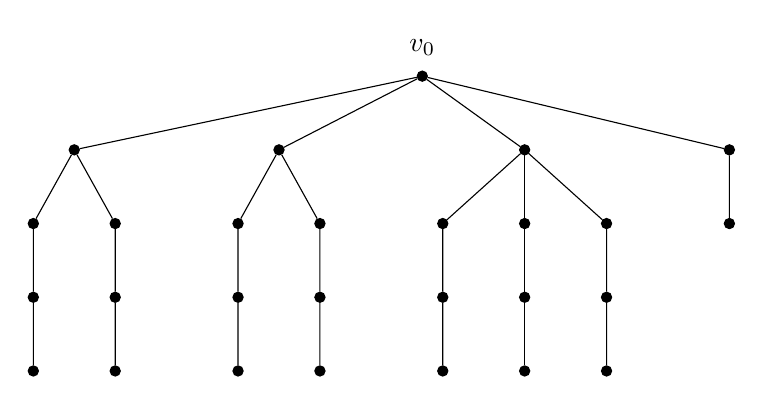
\begin{tikzpicture}[x=0.52cm,y=0.72cm,
  every node/.style={circle,draw,fill=black,inner sep=1.3pt}]
  \node (r) at (10.5,0) {};
  \node (h1) at (2,-1.3) {}; \node (h2) at (7,-1.3) {}; \node (h3) at (13,-1.3) {};
  \node (p1) at (18,-1.3) {}; \node (p2) at (18,-2.6) {};
  \draw (r)--(h1) (r)--(h2) (r)--(h3) (r)--(p1)--(p2);
  \foreach \h/\x in {h1/1,h1/3,h2/6,h2/8,h3/11,h3/13,h3/15}{
    \node (a) at (\x,-2.6) {}; \node (b) at (\x,-3.9) {}; \node (c) at (\x,-5.2) {};
    \draw (\h)--(a)--(b)--(c);
  }
  \node[draw=none,fill=none] at (10.5,0.5) {$v_0$};
\end{tikzpicture}
\caption{The tree $U$ with $27$ vertices.}\label{fig:U}
\end{figure}

\begin{proposition}\label{prop:U}
The tree $U$ satisfies $\gamma(U)=9$ and
\begin{align*}
 D(U,x)={}& 2x^{9}+75x^{10}+2837x^{11}+27278x^{12}+132791x^{13}+403364x^{14}\\
 &+842457x^{15}+1277429x^{16}+1454340x^{17}+1270263x^{18}+862444x^{19}\\
 &+458002x^{20}+190138x^{21}+61213x^{22}+15015x^{23}+2718x^{24}\\
 &+343x^{25}+27x^{26}+x^{27}.
\end{align*}
Since $d_{10}^2=5625<5674=d_{9}d_{11}$, the polynomial $D(U,x)$ is not
log-concave. It is unimodal.
\end{proposition}

\begin{proof}
The polynomial was computed with the recurrence~\eqref{eq:dp} of
Appendix~\ref{app:computation} and confirmed by enumerating all $2^{27}$
subsets of $V(U)$.
\end{proof}

\begin{theorem}\label{thm:unique}
Up to isomorphism, $U$ is the only tree with $27$ vertices whose domination
polynomial is not log-concave.
\end{theorem}

\begin{proof}
This is again the result of the exhaustive computation described in
Appendix~\ref{app:computation}, which covers the $751\,065\,460$ trees with
$27$ vertices.
\end{proof}

\begin{proof}[Proof of Theorem~\ref{thm:smalltrees-intro}]
Part~(i) is Theorem~\ref{thm:small} and Corollary~\ref{cor:smallforest};
part~(ii) is Proposition~\ref{prop:U} and Theorem~\ref{thm:unique}.
\end{proof}

\begin{remark}\label{rem:mechanism}
The failure of log-concavity for $U$ can be traced to the vertex $v_0$. The
dominating sets of $U$ that contain $v_0$ contribute $2$, $75$ and $1141$ to
$d_9$, $d_{10}$ and $d_{11}$, and these three numbers alone satisfy
$75^2\ge2\cdot1141$. A dominating set that avoids $v_0$ has at least two more
vertices than a minimum dominating set; but as soon as it contains a
neighbour $v_i$ of $v_0$, each of the $k_i$ paths attached to $v_i$ can be
dominated by its middle vertex or by its end vertex. There are $1696$
dominating sets of size $11$ that avoid $v_0$, and
$d_{11}=1141+1696=2837$ exceeds $75^2/2$ by less than one per cent. The same
splitting for the tree $T(2,2,3)$, which has $25$ vertices, gives $d_8=1$,
$d_9=37$ and $d_{10}=552+800=1352$, just below $37^2=1369$.
\end{remark}

\begin{remark}\label{rem:family}
Among the trees $T(k_1,\dots,k_r)$ with $r\le5$ and at most $34$ vertices,
exactly six have a non-log-concave domination polynomial: $T(2,3,3)$ of
order $28$; $T(2,3,4)$ and $T(3,3,3)$ of order $31$; and $T(2,3,5)$,
$T(2,4,4)$ and $T(3,3,4)$ of order $34$. For these trees, as for $U$,
log-concavity fails only at the index $\gamma+1$, and the polynomial is
unimodal. In particular the tree $T_3=T(3,3,3)$, which is not covered
by~\cite[Proposition~1]{BS}, is already not log-concave.
\end{remark}


\section{Concluding remarks}\label{sec:remarks}

\subsection*{Gap five}
For $h=5$, Theorem~\ref{thm:criterion-intro} leaves the forests without
isolated vertices that have at most $33$ vertices and satisfy
$n-\gamma\le19$. By Corollary~\ref{cor:smallforest}, a forest of this kind
with a non-unimodal domination polynomial would have a component with at
least $\MinNonLC$ vertices. An exhaustive treatment of the trees with up to
$33$ vertices is out of reach of the programs used here, and
Proposition~\ref{prop:U} shows that log-concavity can no longer be used as
a substitute for unimodality in this range.

\begin{problem}
Prove that the domination polynomial of every forest $F$ with
$\Gamma(F)-\gamma(F)=5$ is unimodal.
\end{problem}

\subsection*{The size of the jumps}
The proof of Theorem~\ref{thm:main} shows that a graph $G$ has a unimodal
domination polynomial as soon as
\begin{equation}\label{eq:jumpquestion}
  c_{j+1}(G)-c_j(G)\le 2\qquad\text{for all } \gamma(G)<j<n ,
\end{equation}
which, by~\eqref{eq:mean}, is the family of inequalities
$(n-j+1)\,d_{j-1}d_{j+1}\le d_jd_{j+1}+(n-j)\,d_j^2$. In the proof of
Lemma~\ref{lem:jump} the variance $v_j$ is bounded by the largest value
compatible with the range of $a(S)$, which could only be attained by a
distribution concentrated on the two extreme values. This crude step is
responsible for the restriction to gaps of order $\sqrt n$.
The inequalities~\eqref{eq:jumpquestion} hold for every tree with at most
$\MaxOrder$ vertices, the largest value of $c_{j+1}-c_j$ over all these trees
being less than $\MaxJumpValue$, and a heuristic search by simulated annealing
among trees with $34$ to $58$ vertices did not produce a value larger than
$1.31$ (supplementary material). Nevertheless they do not hold for all
trees. For $\gamma\le j\le n$ put
\[
  e_j=j-c_j=(n-j+1)\,\frac{d_{j-1}}{d_j},
\]
the average number of non-critical vertices of a dominating set of size $j$;
then $c_{j+1}-c_j=1+e_j-e_{j+1}$ for $\gamma\le j<n$.

\begin{proposition}\label{prop:jumps}
\begin{enumerate}
\item[\textup{(i)}] Let $F$ be a forest of order $n$ and let
$\gamma(F)<j<n$. Then $c_{j+1}-c_j<2\bigl(j-\gamma(F)\bigr)+1$.
\item[\textup{(ii)}] For every integer $t\ge1$ and every $\varepsilon>0$ there
is a tree $T$ such that $c_{j+1}(T)-c_j(T)>2t+1-\varepsilon$ for
$j=\gamma(T)+t$.
\end{enumerate}
In particular, \eqref{eq:jumpquestion} fails for some trees, and the
differences $c_{j+1}-c_j$ are not bounded over all trees.
\end{proposition}

\begin{proof}
(i) By Lemma~\ref{lem:lower}, $j-a(S)\le2(j-\gamma)$ for every
$S\in\Dom_j(F)$, hence $e_j\le2(j-\gamma)$; and $e_{j+1}>0$ because $d_j>0$
and $j<n$.

(ii) Let $r=t+2\ge3$. For integers $k,M\ge1$ let $W$ be the tree obtained from
$T(k,\dots,k)$, with $r$ entries, by attaching to $v_0$ exactly $M$ pendant
paths on two vertices, each joined to $v_0$ by one of its end vertices; it
has $n=1+r+3rk+2M$ vertices. Root $W$ at $v_0$ and
apply~\eqref{eq:dp}. A pendant path on three vertices attached to
$v_i$ has $(A+B+C,\;A+B,\;B)=\bigl(x(x+1)(x+2),\;x(x^2+3x+1),\;x(x+1)\bigr)$
at its end vertex adjacent to $v_i$, and a pendant path on two vertices
attached to $v_0$ has $(A+B+C,\;A+B,\;B)=\bigl(x(x+2),\;x(x+2),\;x\bigr)$.
Writing
\[
  f=x\bigl((x+1)(x+2)\bigr)^k+(x^2+3x+1)^k,\qquad g=f-(x+1)^k,\qquad
  w=(x^2+3x+1)^k-(x+1)^k ,
\]
we obtain $A_{v_i}+B_{v_i}+C_{v_i}=x^kf$, $A_{v_i}+B_{v_i}=x^kg$ and
$B_{v_i}=x^kw$ for $1\le i\le r$, and therefore
\begin{equation}\label{eq:W}
  D(W,x)=x^{rk+M}\Bigl((x+2)^M\bigl(xf^r+g^r\bigr)-w^r\Bigr).
\end{equation}
Here $f(0)=1$, while $g$ and $w$ have zero constant term and linear
coefficients $2^k+2k$ and $2k$. Put $\Phi=(x+2)^Mf^r$ and let $[x^s]\Phi$
denote the coefficient of $x^s$. Since $r\ge3$, \eqref{eq:W} gives
$\gamma(W)=rk+M+1$ and
\begin{equation}\label{eq:Wlow}
  d_{\gamma+s}=[x^s]\Phi\quad(0\le s\le r-2),\qquad
  d_{\gamma+r-1}=[x^{r-1}]\Phi+2^M(2^k+2k)^r-(2k)^r\ \ge\ 2^{M+rk}.
\end{equation}
For $i\ge1$ the coefficient of $x^i$ in $f$ is at most
$2^k\binom{2k}{i-1}+2^i\binom{2k}{i}\le2^k(4k)^i$, because
$(x+1)(x+2)\le2(1+x)^2$ and $x^2+3x+1\le(1+2x)^2$ coefficientwise. Expanding
$f^r$ and noting that at most $\min(i,r)$ factors contribute a positive power
of $x$, we get $[x^i]f^r\le2^{r+i}(4k)^i2^{ki}$ for $1\le i\le r$. From this point assume $M>r-1$, which holds for all sufficiently large $k$
in the choice below. Consequently, for $0\le s\le r-1$,
\[
  [x^s]\Phi=\sum_{i=0}^{s}[x^i]f^r\binom{M}{s-i}2^{M-s+i}
  =\binom Ms2^{M-s}\bigl(1+\theta_s\bigr),\qquad
  0\le\theta_s\le2^r\sum_{i=1}^{s}\Bigl(\frac{16\,k\,s\,2^k}{M-s}\Bigr)^{i},
\]
where we used $\binom{M}{s-i}\big/\binom Ms\le\bigl(s/(M-s)\bigr)^i$. Now let
$k\to\infty$ with $M=2^{k+\lceil k/(2r-2)\rceil}$, so that $k2^k/M\to0$ and
$M^{r-1}/2^{rk}\to0$; then $\theta_s\to0$ for each $s\le r-1$. Let $j=\gamma+t$,
where $t=r-2$, and recall that $n-\gamma=M+2rk+r$. By~\eqref{eq:Wlow},
\[
  e_j=(n-j+1)\frac{d_{\gamma+t-1}}{d_{\gamma+t}}
     =(M+2rk+r-t+1)\,\frac{2t}{M-t+1}\cdot\frac{1+\theta_{t-1}}{1+\theta_t}
     \longrightarrow2t ,
\]
\[
  e_{j+1}=(n-j)\frac{d_{\gamma+t}}{d_{\gamma+t+1}}
     \le(M+2rk+r)\,\frac{M^{t}\,2^{M-t}(1+\theta_t)}{2^{M+rk}}
     \longrightarrow0 .
\]
Hence $c_{j+1}-c_j=1+e_j-e_{j+1}\to2t+1$.
\end{proof}

For $t=1$ the proposition says that $c_{\gamma+2}-c_{\gamma+1}<3$ for every
forest and that the constant $3$ cannot be replaced by a smaller one. The
dominating sets of $W$ of size $\gamma+s$ with $s\le r-2$ are, up to a
negligible proportion, the minimum dominating sets with $s$ further vertices
added on the pendant paths at $v_0$, and each such vertex makes two vertices
non-critical; the far more numerous dominating sets of size $\gamma+r-1$ that
avoid $v_0$ are minimal. Explicitly, the tree obtained from $T(8,8,9)$ by
attaching $3211$ pendant paths on two vertices to $v_0$ has $6501$ vertices
and satisfies $c_{\gamma+2}-c_{\gamma+1}>2$, and for $r=3$, $k=9$ and
$M=7700$ the tree $W$ has $15\,485$ vertices and
$c_{\gamma+2}-c_{\gamma+1}>2.15$. For both trees the complete domination
polynomial was computed from~\eqref{eq:dp}, without the use
of~\eqref{eq:W}; it is unimodal, and \eqref{eq:jumpquestion} fails only for
$j=\gamma+1$ (supplementary material). Trees assembled from the same pieces
are used in~\cite{DHP} for a different purpose: there, a new vertex is joined
to the vertex $v_0$ of each of $m$ copies of $T(k,k,k)$ and to an end vertex
of a path on two vertices, and for large $k$ log-concavity fails at the
indices $\gamma+1,\gamma+3,\dots,\gamma+2m-1$.

The proof of Theorem~\ref{thm:main} uses~\eqref{eq:jumpquestion} only for
indices beyond the increasing segment of Corollary~\ref{cor:segments}(i),
whereas the large jumps of Proposition~\ref{prop:jumps} occur immediately
after $\gamma$. This suggests the following weaker question.

\begin{question}\label{q:jump}
Let $T$ be a tree of order $n$. Does $c_{j+1}(T)-c_j(T)\le2$ hold for every
$j$ with $(n+2\gamma(T)+1)/3<j<n$?
\end{question}

A positive answer would imply the unimodality conjecture for trees, by the
proof of Theorem~\ref{thm:main}. For every tree with at most $26$
vertices, and for the trees $W$ mentioned above, the differences $c_{j+1}-c_j$
in this range are in fact smaller than~$1$ (supplementary material).

At the upper end of this range the answer is positive. Let $T$ be a tree of
order $n\ge5$ with $L$ leaves; then $\gamma(T)\le n/2<n-2$. Clearly
$c_n-c_{n-1}=-c_{n-1}\le0$, and we claim that
\begin{equation}\label{eq:top}
  c_{n-1}-c_{n-2}\le1-\frac2n ,
\end{equation}
with equality if and only if $T$ is a star. A set of vertices is dominating if
and only if its complement contains no closed neighbourhood. The closed
neighbourhoods with two elements are those of the leaves, and they are
pairwise distinct, so $d_{n-2}=\binom n2-L$. Each of them is contained in
$n-2$ sets of three vertices, and a set of three vertices contains at most
two of them, namely when two leaves have the same neighbour. Hence at least
$L(n-2)-\binom L2$ sets of three vertices contain a closed neighbourhood, that
is, $d_{n-3}\le u$ with $u=\binom n3-L(n-2)+\binom L2$. Put $b=d_{n-2}$. Since
$d_{n-1}=n$, \eqref{eq:mean} gives $e_{n-1}=2b/n$ and $e_{n-2}=3d_{n-3}/b$, so
that \eqref{eq:top} is equivalent to $3n\,d_{n-3}\le2b(b-1)$, and
\[
  2b(b-1)-3nu=\tfrac12\,(n-1-L)\bigl(L(3n-4)+n(n-2)\bigr)\ge0 ,
\]
because $L\le n-1$. The right-hand side vanishes only if $L=n-1$, that is,
for the star $K_{1,n-1}$, for which $d_{n-3}=u$.

\subsection*{Beyond forests}
Theorem~\ref{thm:main} applies to every graph satisfying
$(\mathrm{H}_h)$. By Lemma~\ref{lem:upper} and~\eqref{eq:alpha-Gamma}, the upper
bound in~\eqref{eq:H} holds with $h=\Gamma(G)-\gamma(G)$ for every bipartite
graph $G$, so that only the lower bound $a(S)\ge2\gamma(G)-|S|$ is specific to
forests. It fails for $C_4$, but it would be interesting to describe the
bipartite graphs for which it holds.

